\documentclass[12pt]{article}

%% Allows itemranges in enumerations
\def\itemrange#1{%
\addtocounter{enumi}{1}%
\edef\labelenumi{\theenumi--\noexpand\theenumi}%
\addtocounter{enumi}{-1}%
\addtocounter{enumi}{#1}%
\item
\def\labelenumi{\theenumi}}
\renewcommand*{\labelenumi}{\theenumi}

\usepackage{hyperref,graphicx}
\usepackage{fullpage}
\usepackage{enumitem}
\usepackage{subcaption}

\title{RoboCup 2D Half Field Offense \\ Technical Manual}
\author{Matthew Hausknecht}

\begin{document}

\maketitle
\tableofcontents

\section{Overview}

This document describes the installation, usage, state, and action spaces of the HFO domain.

\section{Installation}

Installation with CMake:

\begin{verbatim}
  > mkdir build && cd build
  > cmake -DCMAKE_BUILD_TYPE=Release ..
  > make -j4 # Replace 4 with the number of cores on your machine
  > make install # This just copies binaries to the HFO directory; no sudo required
\end{verbatim}

HFO installation has been tested on Ubuntu Linux and OSX. Successful
installation depends on
\verb+CMake, Boost-system, Boost-filesystem, Flex+. By default, the
soccerwindow2 visualizer is also built and requires
\verb+Qt4+. Experimentally speaking, HFO is fully-functional without
the visualizer. To disable this component, use the following cmake
command:\\

\noindent \verb+  > cmake -DCMAKE_BUILD_TYPE=Release -DBUILD_SOCCERWINDOW=False ..+

\subsection{Python Interface}

The Python interface is required for interfacing Python agents to the
HFO domain. To install this interface, from the main HFO directory:

\noindent \verb+  > pip install .+

or

\noindent \verb+  > pip install --user .+

if you have limited permissions on the machine.

\section{Uninstall}

The install is completely contained in the HFO directory. Simply
delete this directory to uninstall. If you have installed the python
interface, uninstall it as follows: \verb+pip uninstall hfo+.

\begin{figure}[htp]
  \centering
  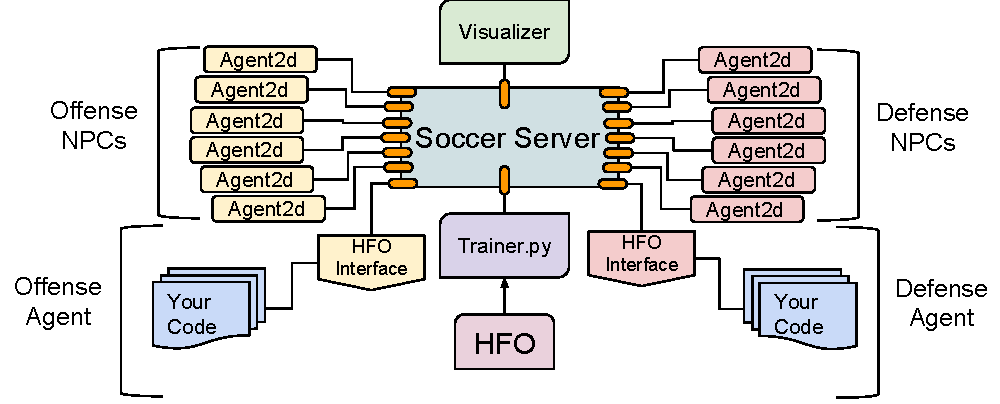
\includegraphics[width=\textwidth]{figures/HFODiagram}
  \caption{HFO is comprised of several components which communicate
    over the network. Network connections are depicted with orange
    ovals. Calling the HFO executable starts the trainer, visualizer,
    and all the offensive and defensive npcs (Agent2d) as well as the
    offensive and defensive agent servers. Your code then uses the HFO
    interface to connect your agent to an agent server. Once all
    servers have connected agents, the game begins. The trainer
    oversees the game and is responsible for resetting the players
    between episodes.}
  \label{fig:hfo}
\end{figure}

\section{Basic Usage}

RoboCup 2D soccer is designed to be played between two teams of
autonomous agents who communicate with a game server. Shown in Figure
\ref{fig:hfo}, the HFO domain reflects these design choices and allows
arbitrary teams to be created consisting of some mix of
non-player-controlled agents (agent2d npcs) and player-controlled
agents. These options are specified through the following flags:\\

\noindent
\verb+ > ./bin/HFO --offense-agents=1 --defense-agents=1 --offense-npcs=2 --defense-npcs=2+\\

This would create a 3v3 game with one player-controlled agent on
each team. In order for the game to start, you must connect your
player-controlled agents to the waiting agent servers. This is done
through the call:\\

\noindent \verb+  > hfo.connectToAgentServer(6000, LOW_LEVEL_FEATURE_SET);+\\
or in Python:\\
\noindent \verb+  > hfo_env.connectToAgentServer(6000, HFO_Features.LOW_LEVEL_FEATURE_SET)+\\

By default, the server for the first agent is allocated to port
6000. Subsequent ports are allocated sequentially backwards (e.g. to
connect the second agent, port 5999 would be used). The default port
may be changed as follows:\\

\noindent \verb+  > ./bin/HFO --port 12345+

\section{Visualizer}

The SoccerWindow2 Visualizer allows a live game to be viewed as it
progresses. By default, the visualizer is enabled. However, the game
will likely proceed at a pace too fast for meaningful watching. To
enforce a standard pace, disable sync-mode:\\

\noindent \verb+  > ./bin/HFO --no-sync+\\

To disable visualization altogether, run in headless mode:\\

\noindent \verb+  > ./bin/HFO --headless+\\

The visualizer may also be used after the end of a game by replaying
logs, as discussed in the next section.

\section{Logging}

By default, the soccer server generates game logs and stores them in
the \verb+log+ directory. The main game log is
\verb+log/incomplete.rcg+. This log may be replayed using the
soccerwindow2 visualizer. \\

\noindent To replay a log: \\
\verb+  > ./bin/soccerwindow2 -l log/incomplete.rcg+

\noindent To disable logging:\\
\verb+  > ./bin/HFO --no-logging +

\noindent To change the logging directory:\\
\verb+  > ./bin/HFO --log-dir /path/to/new/dir +

\section{Recording}

It is possible to record the low-level state perceptions, actions, and
game status of all players:\\

\noindent \verb+  > ./bin/HFO --record + \\

This will produce logs for all the offensive players
(\verb+log/left-[1-11].log+) and defensive players
(\verb+log/right-[1-11].log+). The first offensive player is left-11,
so in the case of single-agent offense, left-11.log will contain the
active player's record. The log, \verb+incomplete.rcg+ may be used to
verify the player numbers on field.

\section{Randomness}

A seed may be specified as follows:\\

\noindent \verb+  > ./bin/HFO --seed 123+\\

This seed will determine the placement of the players and the ball at
the beginning of each episode. Due to non-determinism in the player
policies, it is not sufficient to precisely replicate full games. It
\textit{only} replicates the starting conditions for each episode. The
player's behavior, observations, and physics all proceed
stochastically.

\section{State Spaces}

The HFO domains provides a choice between a low-level feature set and
a higher-level feature set. Selecting between the different feature
sets is accomplished when connecting to the agent server. Also see
\verb|examples/hfo_example_agent.cpp| and
\verb|examples/hfo_example_agent.py| for examples:

\begin{verbatim}
  > hfo.connectToAgentServer(6000, LOW_LEVEL_FEATURE_SET);
  > hfo.connectToAgentServer(6000, HIGH_LEVEL_FEATURE_SET);
\end{verbatim}

\subsection{High Level Feature Set}
A set of high-level features is provided following the example given
by Barrett et al. pp. 159-160 \cite{THESIS14-Barrett}. Barrett writes
``There are many ways to represent the state of a game of half field
offense.  Ideally, we want a compact representation that allows the
agent to learn quickly by generalizing its knowledge about a state to
similar states without over-constraining the policy.'' All features
are encoded a floating point values and normalized to the range of
[-1,1]. Invalid features are given a value of -2. The features are as
follows:

\begin{figure}[htp]
  \centering
  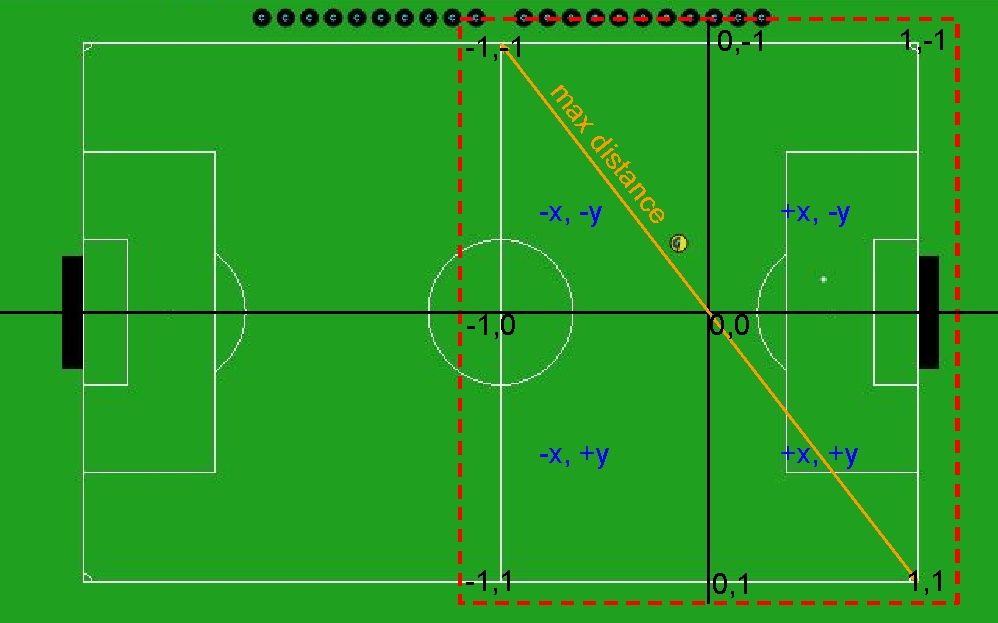
\includegraphics[width=.7\textwidth]{figures/playfieldCoords}
  \caption{\textbf{Normalized Coordinates in the HFO play field}:
    These coordinates are used for reporting the agent's position in
    the high-level feature set as well specifying targets for the
    mid-level actions (Section \ref{sec:mid_level_actions}). The
    red-rectangle shows the boundaries of the reported positions,
    which exceed the play field boundaries by 10\% in each
    direction. Positions exceeding this rectangle are bounded (via
    min/max) to the edges of the rectangle. All distance features are
    normalized against the max HFO distance shown in orange.}
  \label{fig:playfieldCoords}
\end{figure}

\subsubsection{High Level State Feature List}
\begin{enumerate}
\setcounter{enumi}{-1}
\item{\textbf{X position} - The agent’s normalized x-position on the
  field. See Figure \ref{fig:playfieldCoords}.}
\item{\textbf{Y position} - The agent’s normalized y-position on the
  field. See Figure \ref{fig:playfieldCoords}.}
\item{\textbf{Orientation} - The direction that the agent is facing.}
\item{\textbf{Ball Distance} - Normalized distance to the ball.}
\item{\textbf{Ball Angle} - Angle to the ball.}
\item{\textbf{Able to Kick} - Boolean indicating if the agent can kick the ball.}
\item{\textbf{Goal Center Distance} - Normalized distance from the agent to the center of the goal.}
\item{\textbf{Goal Center Angle} - Angle from the agent to the center of the goal.}
\item{\textbf{Goal Opening Angle} - The size of the largest open angle
  of the agent to the goal, shown as $\theta_g$ in Figure
  \ref{fig:openAngle}. Invalid if agent is not playing offense.}
\item [$T$] {\textbf{Teammate i's Goal Opening Angle} - For each
  teammate i: i’s goal opening angle. Invalid if agent is not playing
  offense.}
\item [$1$] {\textbf{Distance to Opponent} - If an opponent is
  present, normalized distance to the closest opponent. This feature
  is absent if there are no opponents.}
\item [$T$] {\textbf{Distance from Teammate i to Opponent} - For each
  teammate i: the normalized distance from the teammate to the closest
  opponent. This feature is absent if there are no opponents. If
  teammates are present but not detected, this feature is considered
  invalid and given the value of -2.}
\item [$T$] {\textbf{Pass Opening Angle} - For each teammate i: the open
  angle available to pass to teammate i. Shown as $\theta_p$ in Figure
  \ref{fig:openAngle}. If teammates are present but not detected, this
  feature is considered invalid and given the value of -2.}
\item [$3T$] {\textbf{Distance, Angle, and Uniform Number of
    Teammates} - For each teammate i: the normalized distance, angle,
  and uniform number of that teammate.}
\end{enumerate}

There are a total of $9 + 5*\textrm{num\_teammates}$ features with an
additional $1 + \textrm{num\_teammates}$ features if at least one
opponent is present.

\begin{figure}[htp]
  \centering
  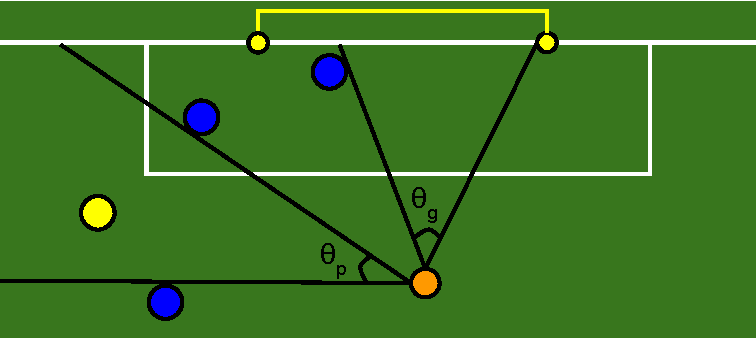
\includegraphics[width=.75\textwidth]{figures/openAngle}
  \caption{Open angle from ball to the goal $\theta_g$ avoiding the
    blue goalie and the open angle from the ball to the yellow
    teammate $\theta_p$. Figure reproduced with permission from Samuel
    Barrett.}
  \label{fig:openAngle}
\end{figure}

\subsection {Low Level Feature Set}
The state features used by HFO are designed with the mindset of
providing an over-complete, basic, egocentric viewpoint. The features
are basic in the sense that they provide distances and angles to
relevant points of interest, but do not include higher level
perceptions such as the largest angle between a goal post and
goalkeeper.

All features are encoded as floating point values normalized to the
range of [-1,1]. Different types of features are discussed next.

\subsubsection{Boolean Features}

Boolean features assume either the minimum feature value of -1 or the
maximum feature value of 1.

\subsubsection{Valid Features}

Since feature information is attained from the Agent's world-model, it
is possible that, the world model's information may be stale or
incorrect. \textit{Valid features} are boolean features indicating
consistency of world model predictions. For example, if the world
model's estimate of the agent's position is known to be flawed, the
\textit{valid feature} for self position would assume the minimum
value of -1. Otherwise it will assume the maximum value of 1.

The features associated with a valid feature are given the value of
zero if an inconsistency is detected. For example, if the world model
detects that the agent's velocity is invalid, the feature that encodes
the magnitude of self velocity will be set to zero.

\subsubsection{Angular Features}

\textit{Angular features} (e.g. the angle to the ball), are encoded as
two floating point numbers -- the $sin(\theta)$ and $cos(\theta)$
where $\theta$ is the original angle in radians. Figure
\ref{fig:ang_example} provides examples of the angular encoding.

This encoding allows the angle to vary smoothly for all possible
angular values. Other encodings such as radians or degrees have a
discontinuity that when normalized, could cause the feature value to
flip between the maximum and minimum value in response to small
changes in $\theta$.

Given an angular feature $\langle \alpha_1, \alpha_2 \rangle$ we can
recover the original angle $\theta$ (in radians) by taking the
$cos^{-1}(\alpha_2)$ and multiplying by the sign of $\alpha_1$.

\begin{figure*}[htp]
  \centering
  \subcaptionbox{Angular Encoding}{
    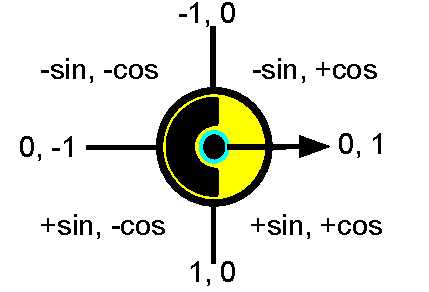
\includegraphics[width=.4\textwidth]{figures/AngExample}
  }
  \hspace{3em}
  \subcaptionbox{Additional Examples}{
    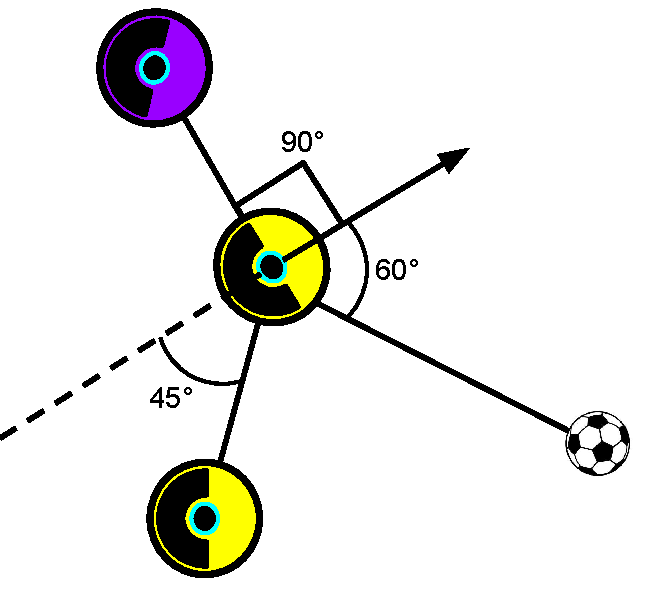
\includegraphics[width=.3\textwidth]{figures/AngFeatExample}
  }
  \caption{\textbf{Angular Encoding:} Objects on the agents left/right
    side result in a negative/positive $sin(\theta)$. $cos(\theta)$ is
    positive in front of the player and negative behind. For example,
    an object directly in front of the player would have angular
    features of $sin(\theta)=0, cos(\theta)=1$. Additional examples:
    \textbf{Angle to ball} $\theta=60^\circ$ or $1.0472$ radians. This
    results in angular features $\langle sin(\theta)=.86,
    cos(\theta)=.49 \rangle$. \textbf{Angle to teammate}:
    $\theta=135^\circ, 2.35$ radians. $\langle sin(\theta)=.71,
    cos(\theta)=-.71 \rangle$. \textbf{Angle to Opponent}:
    $\theta=-90^\circ$ or $-1.57$ radians. $\langle sin(\theta)=-1,
    cos(\theta)=0 \rangle$.}
  \label{fig:ang_example}
\end{figure*}

\subsubsection{Distance Features}

\textit{Distance features} encode the distance to objects of
interest. Unless otherwise indicated, they are normalized against the
maximum possible distance in the HFO playfield (defined as $\sqrt{l^2
  + w^2}$ where $l,w$ are the length and width of the HFO
playfield). A distance of zero will be encoded with the minimum
feature value of -1 while a maximum distance will be encoded with 1.

\subsubsection{Landmark Features}

Landmark features encode the relative angle and distance to a landmark
of interest. Each landmark feature consists of three floating point
values, two to encode the angle to the landmark and one to encode the
distance. Note that if the agent's self position is invalid, then the
landmark feature values are zeroed.

\subsubsection{Player Features}

Player features are used to encode the relationship of the agent to
another player or opponent. Each player feature is encoded as 1) a
landmark feature of that player's location 2) the global angle of that
player's body 3) the magnitude of the player's velocity and 4) the
global angle of the player's velocity. Eight floating point numbers
are used to encode each player feature.

\subsubsection{Other Features}

Some features, such as the agent's stamina, do not fall into any of
the above categories. These features are referred to as \textit{other
  features}.

\subsubsection{Low Level State Feature List}

Basic Features are always present and independent of the number of
teammates or opponents. The 32 basic features are encoded using 58
floating point values (\textit{angular features} require two floats,
\textit{landmark features} require 3). Additionally a variable number
of \textit{player features} are then added. This number depends on the
number of teammates and opponents in the HFO game, but 8 floating
point values are required for each player feature. Thus, the total
number of features is $58 + 8*\textrm{num\_teammates} +
8*\textrm{num\_opponents}$.

\begin{enumerate}
\setcounter{enumi}{-1}
  \item{\textbf{Self\_Pos\_Valid} [Valid] Indicates if self position is valid.}
  \item{\textbf{Self\_Vel\_Valid} [Valid] Indicates if the agent's velocity is valid.}
  \itemrange{1}{\textbf{Self\_Vel\_Ang} [Angle] Angle of agent's velocity.}
  \item{\textbf{Self\_Vel\_Mag} [Other] Magnitude of agent's
    velocity. Normalized against the maximum observed self speed,
    0.46.}
  \itemrange{1}{\textbf{Self\_Ang} [Angle] Agent's Global Body Angle.}
  \item{\textbf{Stamina} [Other] Agent's Stamina: The amount of remaining stamina the
    agent has. Normalized against the maximum observed agent stamina
    of 8000.}
  \item{\textbf{Frozen} [Boolean] Indicates if the agent is Frozen. Frozen status can
    happen when being tackled by another player.}
  \item{\textbf{Colliding\_with\_ball} [Boolean] Indicates if the agent
    is colliding with the ball.}
  \item{\textbf{Colliding\_with\_player} [Boolean] Indicates if the agent
    is colliding with another player.}
  \item{\textbf{Colliding\_with\_post} [Boolean] Indicates if the agent
    is colliding with a goal post.}
  \item{\textbf{Kickable} [Boolean] Indicates if the agent is able to
    kick the ball.}
  \itemrange{2}{\textbf{Goal Center} [Landmark] Center point between the goal posts.}
  \itemrange{2}{\textbf{Goal Post Top} [Landmark] Top goal post.}
  \itemrange{2}{\textbf{Goal Post Bot} [Landmark] Bottom goal post.}
  \itemrange{2}{\textbf{Penalty Box Center} [Landmark] Center of the penalty box line.}
  \itemrange{2}{\textbf{Penalty Box Top} [Landmark] Top corner of the penalty box.}
  \itemrange{2}{\textbf{Penalty Box Bot} [Landmark] Bottom corner of the penalty box.}
  \itemrange{2}{\textbf{Center Field} [Landmark] The left middle point of the
    HFO play area. True center of the full-field.}
  \itemrange{2}{\textbf{Corner Top Left} [Landmark] Top left corner HFO Playfield.}
  \itemrange{2}{\textbf{Corner Top Right} [Landmark] Top right corner HFO Playfield.}
  \itemrange{2}{\textbf{Corner Bot Right} [Landmark] Bot right corner HFO Playfield.}
  \itemrange{2}{\textbf{Corner Bot Left} [Landmark] Bot left corner HFO Playfield.}
  \item{\textbf{OOB Left Dist} [Distance] Distance to the nearest
    point of the left side of the HFO playable area. E.g. distance
    remaining before the agent goes out of bounds in left field.}
  \item{\textbf{OOB Right Dist} [Distance] Distance remaining before
    the agent goes out of bounds in right field.}
  \item{\textbf{OOB Top Dist} [Distance] Distance remaining before
    the agent goes out of bounds in top field.}
  \item{\textbf{OOB Bot Dist} [Distance] Distance remaining before
    the agent goes out of bounds in bottom field.}
  \item{\textbf{Ball Pos Valid} [Valid] Indicates if the ball position estimate is valid.}
  \itemrange{1}{\textbf{Ball Angle} [Angle] Angle to the ball from the agent's perspective.}
  \item{\textbf{Ball Dist} [Distance] Distance to the ball.}
  \item{\textbf{Ball Vel Valid} [Valid] Indicates if the ball velocity estimate is valid.}
  \item{\textbf{Ball Vel Mag} [Other] Global magnitude of the ball velocity. Normalized against the observed maximum ball velocity, 3.0.}
  \itemrange{1}{\textbf{Ball Vel Ang} [Angle] Global angle of ball velocity.}
  \item [$8T$] {\textbf{Teammate Features} [Player] One teammate feature set (8 features) for each teammate active in HFO, sorted by proximity to the agent.}
  \item [$8O$] {\textbf{Opponent Features} [Player] One opponent feature set (8 features) for each opponent present, sorted by proximity to the player.}
\end{enumerate}

\section{Action Space}
The HFO domain provides support for both low-level primitive actions
and high-level strategic actions. Basic, parameterized actions are
provided for locomotion and kicking. Additionally high-level strategic
actions are available for moving, shooting, passing and
dribbling. Control of the agent's head and gaze is not provided and
follows Agent2D's default strategy. Both low and high level actions
are available through the same interface. It is the responsibility of
the user to faithfully report which action spaces were used.

\subsection{Low Level Actions}
\label{sec:low_level_actions}
\begin{itemize}
\item{\textbf{Dash}(power, degrees): Moves the agent with power [-100,
    100] where negative values move backwards. The relative direction
  of movement is given in degrees and varies between [-180,180] with 0
  degrees being a forward dash and 90 degrees dashing to the agent's
  right side. Note, dashing does not turn the agent.}
\item{\textbf{Turn}(degrees): Turns the agent in the
  specified direction. Valid values range between [-180, 180] degrees
  where 90 degrees turns the agent to directly to its right side.}
\item{\textbf{Tackle}(degrees): Contest the ball. Direction
  varies between [-180, 180].}
\item{\textbf{Kick}(power, degrees): Kick the ball with power [0, 100]
  in relative direction [-180, 180]. Has no effect if the agent does
  not possess the ball.}
\end{itemize}

\subsection{Mid Level Actions}
\label{sec:mid_level_actions}
\begin{itemize}
\item{\textbf{Kick$\_$To}(target$_x$, target$_y$, speed): Kicks the
  ball to the specified target point with the desired speed. Valid
  values for target$_{x,y} \in [-1,1]$ and speed $\in [0,3]$.}
\item{\textbf{Move$\_$To}(target$_x$, target$_y$): Moves to the
  specified target point using the max dash speed. Valid values for
  target$_{x,y} \in [-1,1]$.}
\item{\textbf{Dribble$\_$To}(target$_x$, target$_y$): Dribbles the
  ball to the specified target point. Attempts to fetch the ball if
  the agent doesn't already possess it. Performs some checks to avoid
  opponents and keeps good control of the ball. Valid values for
  target$_{x,y} \in [-1,1]$.}
\item{\textbf{Intercept}(): Moves to intercept the ball, taking into
  account the ball velocity. More efficient than chasing the ball.}
\end{itemize}

\subsection{High Level Actions}
\label{sec:high_level_actions}
\begin{itemize}
\item{\textbf{Move}(): Re-positions the agent according to the
  strategy given by Agent2D. The \textit{move} command works only when
  agent does not have the ball. If the agent has the ball, another
  command such as \textit{dribble}, \textit{shoot}, or \textit{pass}
  should be used.}
\item{\textbf{Shoot}(): Executes the best available shot. This command
  only works when the agent has the ball.}
\item{\textbf{Pass}(teammate\_uniform\_number): Passes to the teammate
  with the provided uniform number. Does nothing if the player does
  not have control of the ball or the requested teammate is not
  detected.}
\item{\textbf{Dribble}(): Advances the ball towards the goal using a
  combination of short kicks and moves.}
\end{itemize}

\subsection{Special Actions}
\begin{itemize}
\item{\textbf{NO-OP}: Indicates that the agent should take no action.}
\item{\textbf{Quit}: Indicates to the agent server that you wish to
  terminate the HFO environment.}
\end{itemize}

\section{Developing a New Agent}

New agents may be developed in C++ or Python. In Python, as long as
the hfo interface has been installed, the agent needs only to
\verb+from hfo import *+. In C++ it is necessary to
\verb+#include <HFO.hpp>+ and also to link against the shared object
library \verb+lib/libhfo.so+ when compiling:\\

\begin{verbatim}
  > g++ example/your_new_agent.cpp -I src -L lib -Wl,-rpath=lib -lhfo
\end{verbatim}

\bibliographystyle{abbrv}
\bibliography{manual}

\end{document}
